\documentclass[12pt]{report}
\usepackage[utf8]{inputenc}
\usepackage{cite}
\usepackage[hidelinks]{hyperref}
\usepackage{graphicx}
\usepackage{amsfonts}
\usepackage{mathtools}
\usepackage{caption}
\usepackage{fancyhdr}

\pagestyle{fancy}
\fancyhf{}
\rhead{5-stage Pipelined Processor Design Report}
\lhead{\thesection}
\rfoot{\thepage}

\DeclarePairedDelimiter\ceil{\lceil}{\rceil}
\DeclarePairedDelimiter\floor{\lfloor}{\rfloor}

\title{\textbf{5-stage Pipelined Processor Design Report}\\Team \#4}
\author{
  Mohamed Shawky\\
  \small\texttt{SEC:2, BN:16}
  \and
  Remonda Talaat\\
  \small\texttt{SEC:1, BN:20}
  \and
  Evram Youssef\\
  \small\texttt{SEC:1, BN:9}
  \and
  Mahmoud Adas\\
  \small\texttt{SEC:2, BN:21}
}
\date{\today}

\begin{document}

\thispagestyle{empty}

\maketitle
\tableofcontents
\listoffigures
\listoftables
\clearpage

\pagenumbering{arabic}

%%%%%%%%%%%%%%%%%%%%%%%%%%%%%%%%%%%%%%%%%%%%%%%%%%%%%%%%%%%%%%%%%%%%%%%%%%%%%%%%%%%%%%%%%%%%%%%%%%%%%%%%%%%%%%%%%%%%%%%%%%%
\part{Introduction}

\section{Abstract}
This report describes our design work of the 5-stage pipelined processor, that follows Harvard architecture.

This report contains:
\begin{itemize}
    \item the overall system blocks and connections.
    \item the functionalities of the different blocks.
    \item the hazard solutions.
\end{itemize}

\section{Task Distribution}
Table \ref{tab:td} contains the task distribution.

\begin{center}
    \captionof{table}{Task Distribution\label{tab:td}}
 \begin{tabular}{||c| p{100mm}||} 
 \hline
 Team Member & Tasks \\ [0.5ex] 
 \hline\hline
 Mohamed Shawky & -- Overall system design. \newline -- Hazard detection and handling. \newline -- Document typing and formatting. \\
 \hline
 Remonda Talaat & -- Instruction format. \newline -- Interrupt Handling. \newline -- Overall system design. \\
 \hline
 Evram Youssef & -- Control unit and its signals. \newline -- Low level block design. \newline -- Pipeline buffers. \\
 \hline
 Mahmoud Adas & -- Low level block design. \newline -- Pipeline buffers. \newline -- Document typing and formatting. \\ 
 \hline
\end{tabular}
\end{center}

%%%%%%%%%%%%%%%%%%%%%%%%%%%%%%%%%%%%%%%%%%%%%%%%%%%%%%%%%%%%%%%%%%%%%%%%%%%%%%%%%%%%%%%%%%%%%%%%%%%%%%%%%%%%%%%%%%%%%%%%%%%
\part{Overall System Design}
\section{Overall System Design Schema}
Figure \ref{fig:overall} shows the overall system design in detail. Each unit is described in details in its section.
\begin{center}
    \begin{figure}[hp]
        \centering
        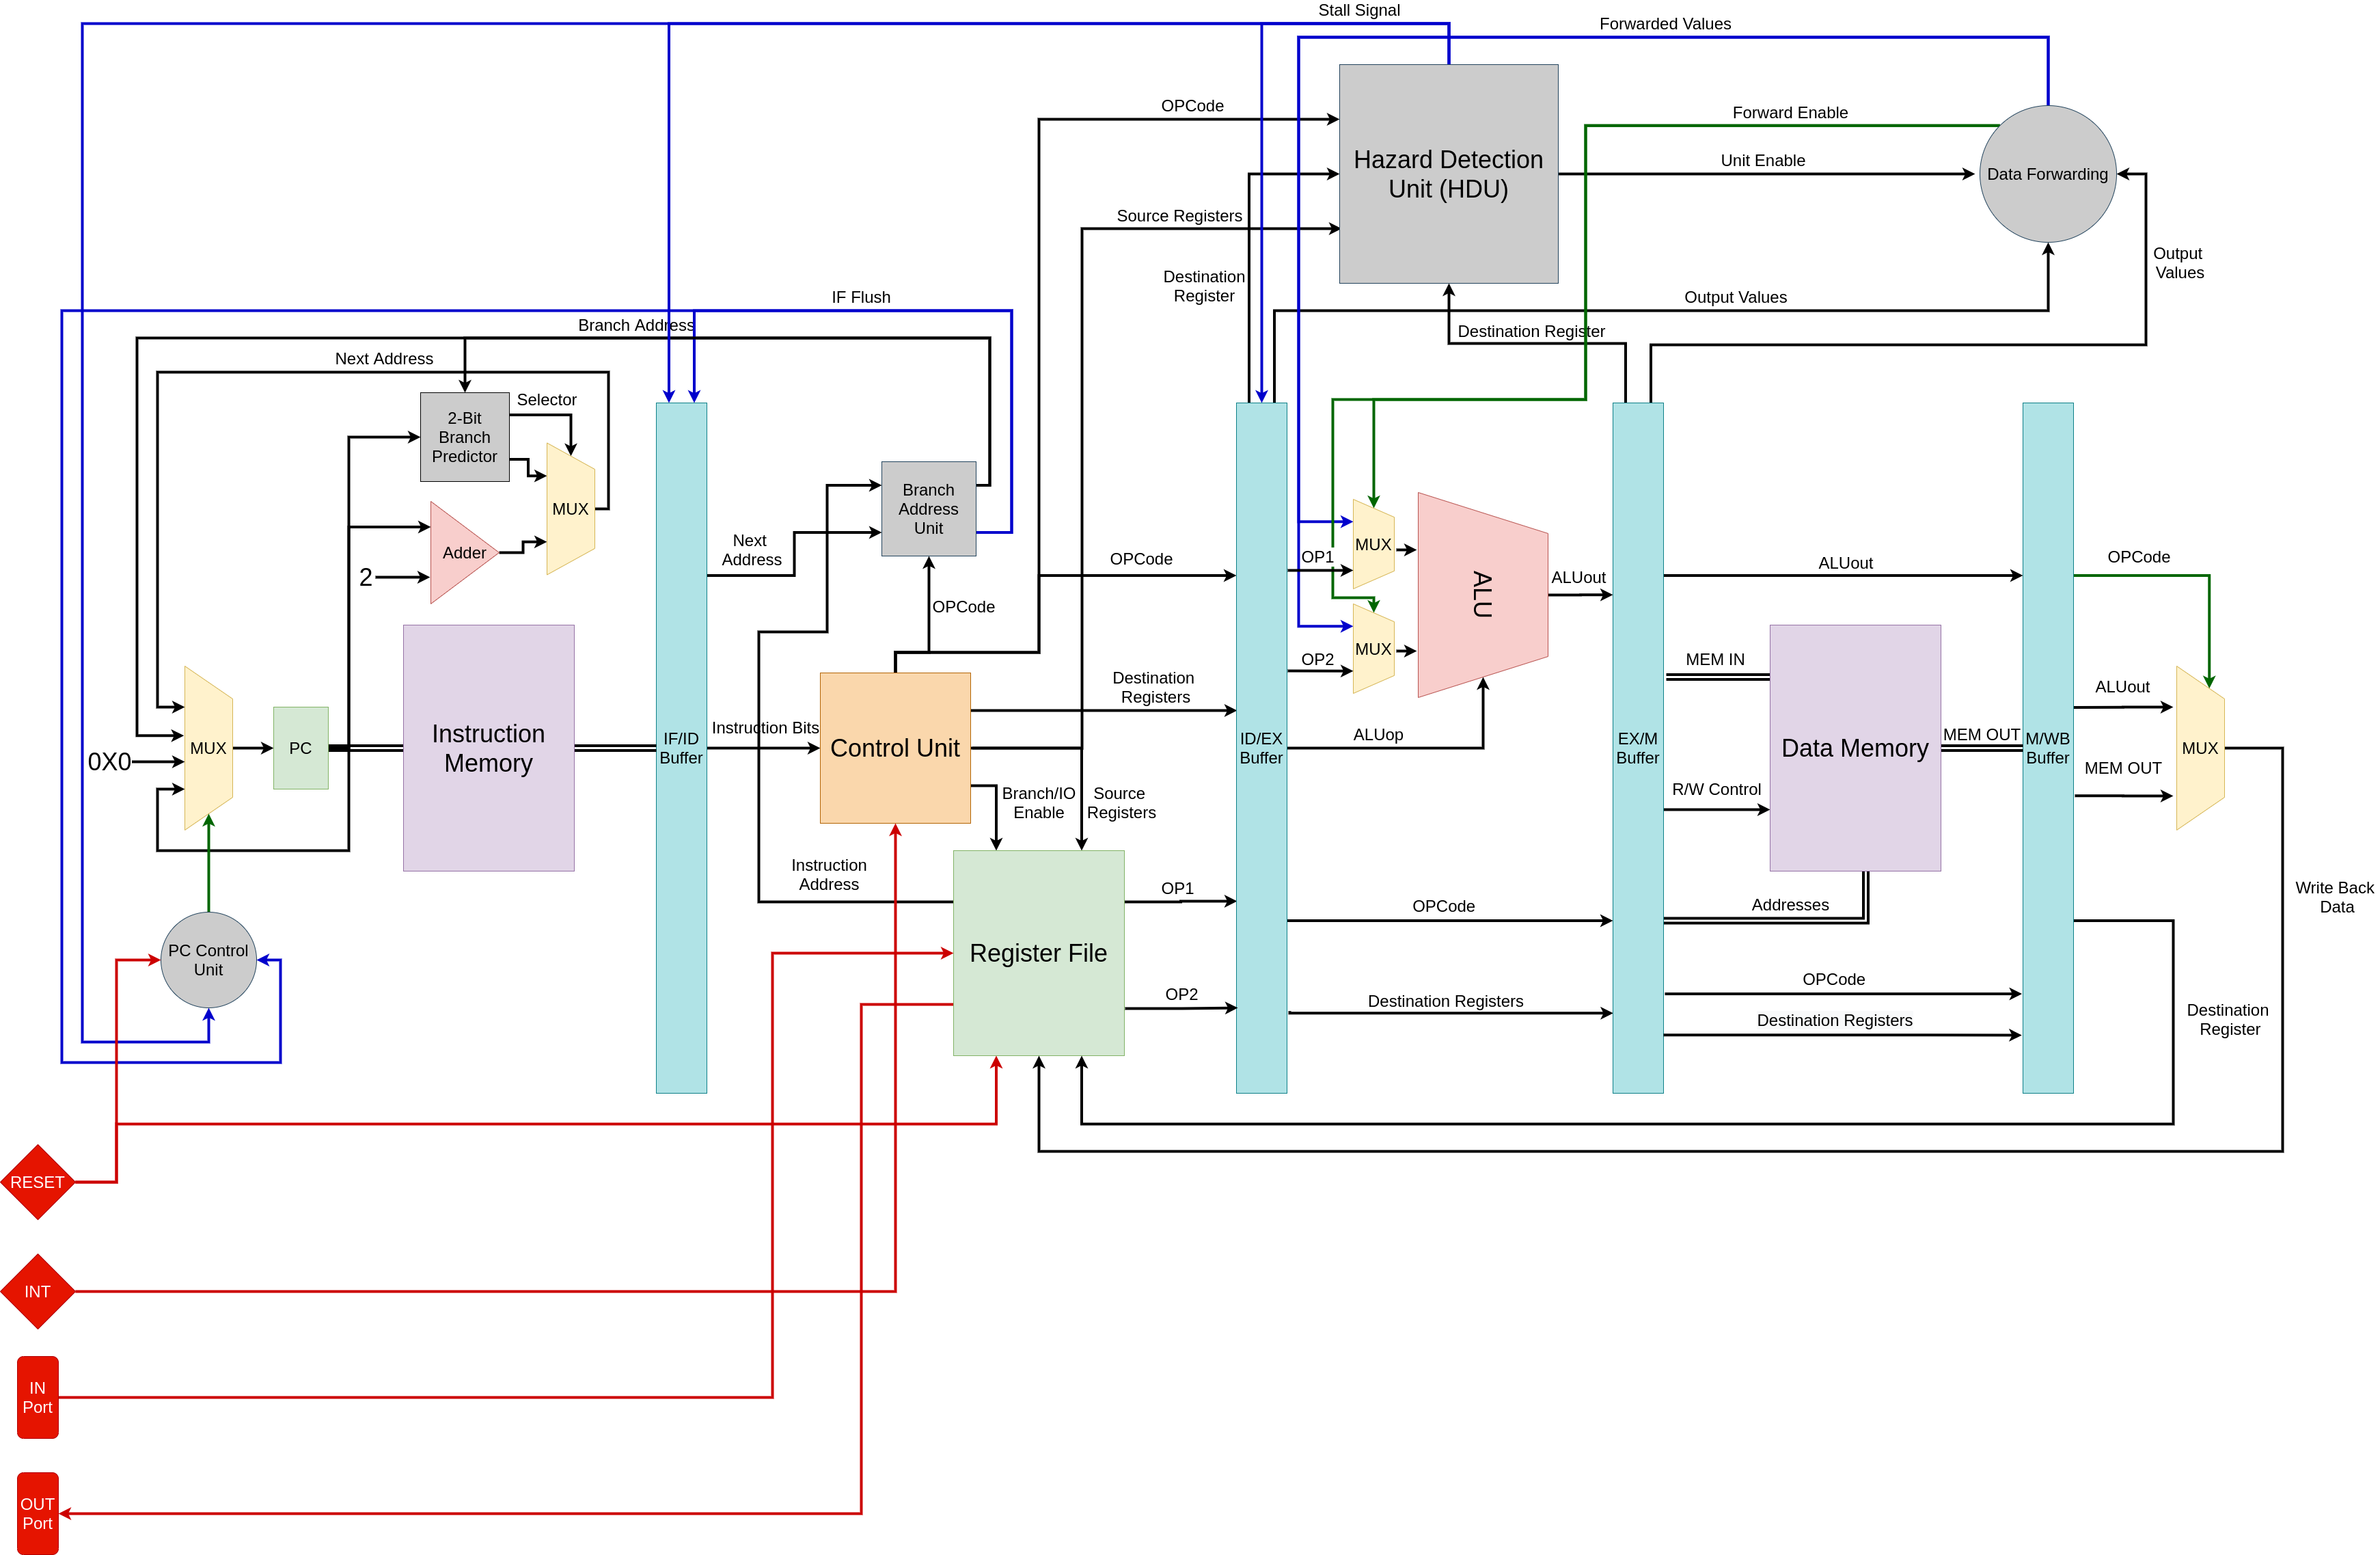
\includegraphics[width=\textwidth]{overall_system}
        \caption{Overall System Design}
        \label{fig:overall}
    \end{figure}
\end{center}

\section{Memory Specs}
Because the design follows Harvard architecture, it uses 2 separate memory units, one for instructions and another one for both the data and stack.
\begin{itemize}
    \item Instructions Memory:
    \begin{itemize}
        \item 2$^{32}$ $\times$ 16 bits
        \item 16-bit bus
    \end{itemize}
    \item Data Memory:
    \begin{itemize}
        \item 2$^{32}$ $X$ 16 bits
        \item 32-bit bus
        \item SP starts at 2$^{32}$-1
    \end{itemize}
\end{itemize}

\section{PC Control Unit}

\subsection{Inputs}
\begin{itemize}
    \item IF Flush (1 bit)
    \item Stall Signal (1 bit)
    \item RESET Signal (1 bit)
    \item Interrupt Signal (1 bit)
    \item Current OPCode (7 bits)
\end{itemize}

\subsection{Outputs}
\begin{itemize}
    \item PC Mux Selectors (3 bits)
\end{itemize}

\subsection{Logic}
\begin{itemize}
    \item If IF Flush == 1, Output = 001
    \item If RESET == 1, Output = 010
    \item If Stall == 1, Output = 011
    \item If Interrupt == 1 $||$ OPCode == RET/RTI, Output = 100
    \item Else, Output = 000
\end{itemize}

\section{Dynamic Branch Prediction}
Figure \ref{fig:bpu} shows the branch prediction unit.
\begin{center}
    \begin{figure}[hp]
        \centering
        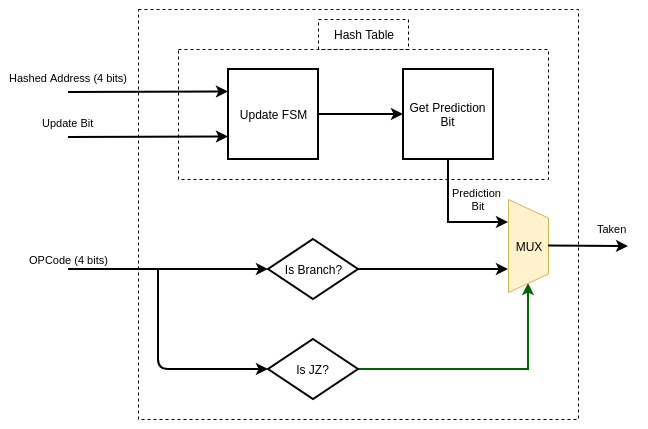
\includegraphics[width=0.8\textwidth]{bpu}
        \caption{Branch Prediction Unit Diagram}
        \label{fig:bpu}
    \end{figure}
\end{center}

\subsection{Inputs}
\begin{itemize}
    \item Hashed Address (4 bits)
    \item Update Bit (1 bit): \emph{Taken or Not}  to update FSM
    \item OPcode (4 bits)
\end{itemize}

\subsection{Outputs}
\begin{itemize}
    \item Taken (1 bit): predict whether the branch taken or not
\end{itemize}

\subsection{Logic}
\begin{itemize}
    \item Updates the FSM corresponding to the hashed address.
    \item Checks whether the OPCode is of a conditional branch instruction.
    \item Outputs the prediction bit \emph{(Taken or Not)} accordingly.
\end{itemize}

\section{Stack Pointer (SP) Peak Unit}
Figure \ref{fig:pspu} shows the stack pointer unit.

\subsection{Inputs}
\begin{itemize}
    \item Current SP (32 bits)
    \item Prev OPCodes (3$X$7 bits)
\end{itemize}

\subsection{Outputs}
\begin{itemize}
    \item Expected SP (32 bits): stack pointer to read from after eliminating hazards
\end{itemize}

\begin{center}
    \begin{figure}[hp]
        \centering
        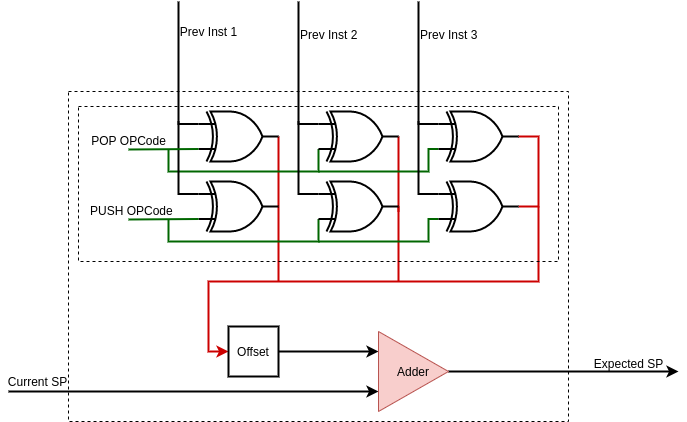
\includegraphics[width=0.8\textwidth]{pspu}
        \caption{Stack Pointer (SP) Peak Unit Diagram}
        \label{fig:pspu}
    \end{figure}
\end{center}

\subsection{Logic}
This unit peaks the value of the stack pointer on returning from a subroutine or an interrupt, in order to calculate the correct value of the address from which the original program counter read from memory. It checks for \emph{POP/PUSH} instructions and use the count to update the address.

\textbf{NOTE:} In case we didn't use this unit, we will stall the pipe for three consecutive cycles to eliminate possible hazards.

\section{Branch Address Unit}
Figure \ref{fig:bau} shows the branch address unit.
\begin{center}
    \begin{figure}[hp]
        \centering
        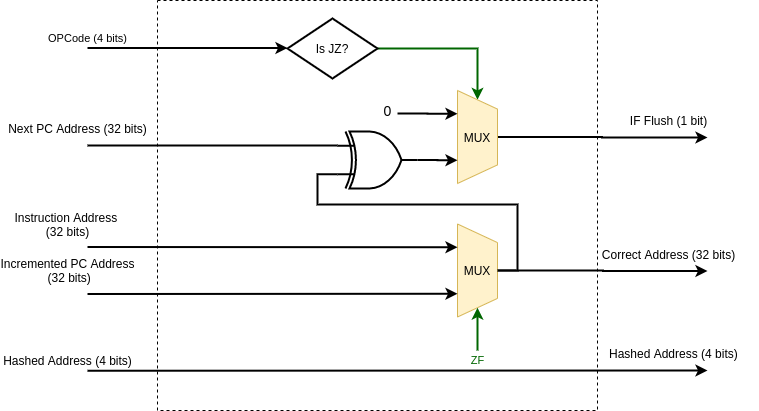
\includegraphics[width=0.8\textwidth]{bau}
        \caption{Branch Address Unit Diagram}
        \label{fig:bau}
    \end{figure}
\end{center}

\subsection{Inputs}
\begin{itemize}
    \item Next PC Address (32 bits)
    \item Instruction Address (32 bits)
    \item Incremented PC Address (32 bits)
    \item Hashed Address (4 bits)
    \item OpCode (4 bits)
\end{itemize}

\subsection{Outputs}
\begin{itemize}
    \item IF Flush (1 bit)
    \item Branch Address (32 bits)
    \item Hashed Address (4 bits)
\end{itemize}

\subsection{Logic}
\begin{itemize}
    \item Check if OpCode is of a conditional branch instruction, if true:
    \begin{itemize}
        \item Check whether PC Next Address is equal to Instruction Address
        \item If true:
        \begin{itemize}
            \item IF Flush = 0, Branch Address = Instruction Address
        \end{itemize}
        \item If false:
        \begin{itemize}
            \item IF Flush = 1, Branch Address = Instruction Address
        \end{itemize}
    \end{itemize}
\end{itemize}

\section{Register File}
Figure \ref{fig:reg_file} shows the register file.

\subsection{Registers}
\begin{itemize}
    \item 8 general purpose registers
    \item Stack pointer (SP) register
    \item Program counter (PC) register
\end{itemize}

\subsection{Inputs}
\begin{itemize}
    \item Dest Regs: 2$X$4 bits (for destination selection)
    \item SRC Regs: 2$X$4 bits (for source selection)
    \item Fetch Reg: 4 bits (for fetch branch register selection)
    \item WB values: 2$X$32 bits (for write back values)
    \item RESET: 1 bit (for registers clear).
    \item Branch/IO: 2 bits (to determine whether the operation is IO or branch)
    \item IN Port: 32 bits (IO input port)
\end{itemize}

\subsection{Outputs}
\begin{itemize}
    \item OP1: 32 bits (value of first operand)
    \item OP2: 32 bits (value of second operand)
    \item Fetch Value: 32 bits (value of branch address required by fetch)
    \item Instruction Address: 32 bits (value of branch address)
    \item OUT Port: 32 bits (IO output port)
\end{itemize}

\subsection{Logic}
The register selector acts like a decoder to select the required operation and the register on which the operation performed.

\begin{center}
    \begin{figure}[hp]
        \centering
        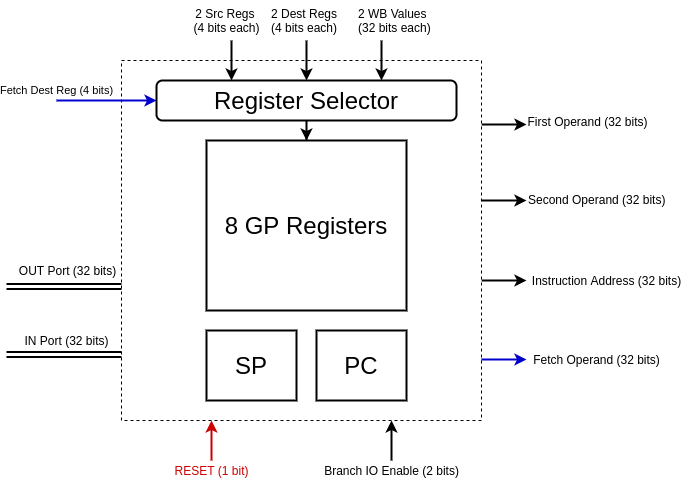
\includegraphics[width=0.8\textwidth]{reg_file}
        \caption{Register File Diagram}
        \label{fig:reg_file}
    \end{figure}
\end{center}

\section{ALU}

\subsection{Inputs}
\begin{itemize}
    \item ALUop: 4 bits (refer to ALU Operations below)
    \item Operands: 2$X$32 bits (2 input operands)
\end{itemize}

\subsection{Outputs}
\begin{itemize}
    \item ALUout: 32 bits (operation result)
\end{itemize}

\subsection{ALU Operations}
\begin{itemize}
    \item 0000 $-$ NOP $-$ (no operation)
    \item 0001 $-$ INC $-$ (first operand + 1)
    \item 0010 $-$ DEC $-$ (first operand - 1)
    \item 0011 $-$ ADD $-$ (first operand + second operand)
    \item 0100 $-$ SUB $-$ (first operand - second operand)
    \item 0101 $-$ AND $-$ (first operand \&\& second operand)
    \item 0110 $-$ OR $-$ (first operand $||$ second operand)
    \item 0111 $-$ NOT $-$ (!first operand)
    \item 1000 $-$ SHL $-$ (shift first operand to the left)
    \item 1001 $-$ SHR $-$ (shift first operand to the right)
    \item 1010 $-$ INC2 $-$ (first operand + 2)
    \item 1011 $-$ DEC2 $-$ (first operand - 2)
    \item 1100 $-$ INC4 $-$ (first operand + 4)
    \item 1101 $-$ DEC4 $-$ (first operand - 4)
\end{itemize}

\subsection{Logic}
\begin{itemize}
    \item ALU performs the operation and changes the CCR accordingly.
    \item The input operands of the ALU are multiplexed between forwarded data and register data, with selectors from data forwarding unit.
\end{itemize}

%%%%%%%%%%%%%%%%%%%%%%%%%%%%%%%%%%%%%%%%%%%%%%%%%%%%%%%%%%%%%%%%%%%%%%%%%%%%%%%%%%%%%%%%%%%%%%%%%%%%%%%%%%%%%%%%%%%%%%%%%%%
\part{Instruction Format}

\section{One Operand Operations}
\begin{itemize}
    \item 4 bits (1111) for one operand instructions.
    \item 3 bits to define instruction.
    \item 3 bits for destination register.
    \item 1 bit to define the memory slots occupied by the instruction.
    \item Total of 11 bits, padded with 5 0's to fit 16 bits.
\end{itemize}
\begin{center}
    \captionof{table}{One Operand Instruction Mapping\label{tab:1op}}
 \begin{tabular}{||c| c| c| c| p{40mm}||} 
 \hline
 Operation & OpCode & Destination & 16$|$32 & Conditions  \\ [0.5ex] 
 \hline\hline
 IN & 1111000 & 000:111 & 0 & ----------------------- \\
 \hline
 NOT & 1111001 & 000:111 & 0 & if !Rdst=0,Z=1 \newline if !Rdst$<$0,N=1 \\
 \hline
 INC & 1111010 & 000:111 & 0 & if Rdst+1=0,Z=1 \newline if Rdst+1$<$0,N=1 \\
 \hline
 DEC & 1111011 & 000:111 & 0 & if Rdst-1=0,Z=1 \newline if Rdst-1$<$0,N=1 \\
 \hline
 OUT & 1111100 & 000:111 & 0 & ----------------------- \\
 \hline
\end{tabular}
\end{center}

\section{Special Operations}
\begin{itemize}
    \item 16 0's to represent NOP (0000000000000000).
\end{itemize}

\section{Two Operand Operations}
\begin{itemize}
    \item 4 bits to define instruction.
    \item 3 bits for each of Rsrc1, Rsrc2 and Rdst.
    \item 1 bit to define the memory slots occupied by the instruction.
    \item 16 bits for immediate values.
    \item Total of 14 bits in most cases with some exceptions mentioned below.
\end{itemize}
\begin{center}
    \captionof{table}{Two Operand Instruction Mapping\label{tab:1op}}
 \begin{tabular}{||c| c| c| c| c| c| c| p{30mm}||} 
 \hline
 Operation & OpCode & Rsrc1 & Rsrc2 & Rdst & imm & 16$|$32 & Conditions  \\ [0.5ex] 
 \hline\hline
 SWAP & 0001 & 000:111 & --- & 000:111 & --- & 0 & ----------------------- \\
 \hline
 ADD & 0010 & 000:111 & 000:111 & 000:111 & --- & 0 & if Result=0,Z=1 \newline if Result$<$0,N=1 \\
 \hline
 SUB & 0011 & 000:111 & 000:111 & 000:111 & --- & 0 & if Result=0,Z=1 \newline if Result$<$0,N=1 \\
 \hline
 AND & 0100 & 000:111 & 000:111 & 000:111 & --- & 0 & if Result=0,Z=1 \newline if Result$<$0,N=1 \\
 \hline
 OR & 0101 & 000:111 & 000:111 & 000:111 & --- & 0 & if Result=0,Z=1 \newline if Result$<$0,N=1 \\
 \hline
 SHL & 0110 & 000:111 & --- & --- & 16 bits & 1 & update carry flag \\
 \hline
 SHR & 0111 & 000:111 & --- & --- & 16 bits & 1 & update carry flag \\
 \hline
 IADD & 1000 & 000:111 & --- & 000:111 & 16 bits & 1 & if Result=0,Z=1 \newline if Result$<$0,N=1 \\
 \hline
\end{tabular}
\end{center}

\section{Memory Operations}
\begin{itemize}
    \item 4 bits to define instruction.
    \item 3 bits for destination register.
    \item 1 bit to define the memory slots occupied by the instruction.
    \item 16 bits for immediate values.
    \item 20 bits for effective addresses.
    \item Total of 8 bits with no immediate values or effective addresses.
    \item Total of 24 bits with immediate values.
    \item Total of 28 bits with effective addresses.
\end{itemize}
\begin{center}
    \captionof{table}{Memory Instruction Mapping\label{tab:1op}}
 \begin{tabular}{||c| c| c| c| c| c| p{40mm}||} 
 \hline
 Operation & OpCode & Rdst & imm & EA & 16$|$32 & Conditions  \\ [0.5ex] 
 \hline\hline
 PUSH & 1001 & 000:111 & --- & --- & 0 & ----------------------- \\
 \hline
 POP & 1010 & 000:111 & --- & --- & 0 & ----------------------- \\
 \hline
 LDM & 1011 & 000:111 & 16 bits & --- & 1 & ----------------------- \\
 \hline
 LDD & 1100 & 000:111 & --- & 20 bits & 1 & ----------------------- \\
 \hline
 STD & 1101 & 000:111 & --- & 20 bits & 1 & ----------------------- \\
 \hline
\end{tabular}
\end{center}

\section{Branch and Change Control Operations}
\begin{itemize}
    \item 4 bits (0000) for branching instructions.
    \item 3 bits to define instruction.
    \item 3 bits for destination register.
    \item 1 bit to define the memory slots occupied by the instruction.
    \item Total of 11 bits, padded with 5 0's to fit 16 bits. 
\end{itemize}
\begin{center}
    \captionof{table}{One Operand Instruction Mapping\label{tab:1op}}
 \begin{tabular}{||c| c| c| c| p{40mm}||} 
 \hline
 Operation & OpCode & Destination & 16$|$32 & Conditions  \\ [0.5ex] 
 \hline\hline
 JZ & 0000001 & 000:111 & 0 & ----------------------- \\
 \hline
 JMP & 0000010 & 000:111 & 0 & ----------------------- \\
 \hline
 CALL & 0000011 & 000:111 & 0 & ----------------------- \\
 \hline
 RET & 0000100 & --- & 0 & ----------------------- \\
 \hline
 RTI & 0000101 & --- & 0 & ----------------------- \\
 \hline
\end{tabular}
\end{center}

%%%%%%%%%%%%%%%%%%%%%%%%%%%%%%%%%%%%%%%%%%%%%%%%%%%%%%%%%%%%%%%%%%%%%%%%%%%%%%%%%%%%%%%%%%%%%%%%%%%%%%%%%%%%%%%%%%%%%%%%%%%
\part{Control Unit (Signals)}

\section{Overview}
Control unit is responsible for generating the control signals that are used to activate several operations throughout the pipeline. Also, it's responsible for the extraction of specific information from instruction bits.

\begin{itemize}
    \item It communicates with:
    \begin{itemize}
        \item IF/ID buffer: for reading the instruction bits.
        \item ID/EX buffer: for writing the appropriate registers, ALUop and signals.
        \item Register file: for selecting the registers needed to be read (Rsrc1 and Rsrc2).
        \item Hazards units (HDU and Branch Address Unit): for sending enables and needed signals.
    \end{itemize}
    
    \item Unit Interface:
    \begin{itemize}
    
        \item Inputs: 
        \begin{itemize}
            \item Instruction Bits (32 bits)
            \item Interrupt bit (1 bit)
        \end{itemize}
        
        \item Outputs:
        \begin{itemize}
            \item Rsrc2\_val (32 bits) for immediate values or effective addresses
            \item Rsrc1\_sel (4 bits)
            \item Rsrc2\_sel (4 bits)
            \item Rdst1\_sel (4 bits)
            \item Rdst2\_sel (4 bits) used only in case of swap
            \item Branch/IO Enable (2 bits)
            \item OP2\_sel (1 bit)
            \item SP Enable (1 bit)
            \item OpCode (7 bits)
            \item Branch Enable (1 bit)
            \item ALUop (4 bits)
            \item R/W Control Signal (2 bits)
        \end{itemize}
        
    \end{itemize}
    
    \item Interpretation:
    \begin{itemize}
        \item \textbf{Rsrc2\_val (32 bits):} occupies a single place in the ID/EX buffer. However, it's used in many different ways. It can be used as a register value extracted form register file. it can be used as an immediate value extracted from IF/ID buffer. Also, it can hold the stack pointer address, as well as the effective address (EA) sent to the memory for reading or writing.
        \item \textbf{Rdst2 (4 bits):} only used when dealing with a SWAP instruction, thus we need Op1 and Op2 and their new selectors.
        \item \textbf{OP2\_sel (1 bit):} determines the value of Rsrc2 register in ID/EX buffer, whether it's immediate or register value.
        \item  \textbf{Branch/IO Enable (2 bits):} informs the register file what operation of these are we executing (No/In/Out/Branch), however \emph{Branch Enable} (1 bit) interacts with the Branch Address Unit, informing it what type of OpCode are we dealing with (branching or not).
    \end{itemize}
\end{itemize}

\section{Control Signals}
In this section, instructions are divided into seven types based on the signals produced:
\begin{itemize}
    \item One Operand (not,inc,dec,out,in).
    \item Two Operands (add,sub,and,or).
    \item Immediate Operand (iadd,shl,shr,ldm).
    \item Data (ldd,std).
    \item Stack (push,pop,call,ret,rti).
    \item Jump (jz, jmp).
    \item Special (nop,swap,reset,int).
\end{itemize}   

\subsection{One Operand Instructions}
\begin{itemize}
    \item IB[31:0] are the instruction bits.
    \item Inserting (1111) to Rsrc/Rdst selectors informs the register file not to output any register values.
    \item 'x' indicates don't care.
    \item 0000 at the ALUop indicates no operation.
    \item Rsrc1\_sel is the same as Rdst1\_sel.
\end{itemize}

\begin{center}
    \captionof{table}{One Operand Instruction Control Signals Part I\label{tab:1op1}}
\begin{tabular}{||p{20mm}| p{15mm}| p{15mm}| p{15mm}| p{15mm}| p{15mm}| p{15mm}||} 
\hline
Instruction & OPCode & ALUop & Rsrc1 selector & Rsrc2 selector & Rdst1 selector & Rsrc2 value \\ [0.5ex] 
\hline\hline
NOT & IB[31:25] & 0111 & 0 and IB[24:22] & 1111 & 0 and IB[24:22] & x  \\
\hline
INC & IB[31:25] & 0001 & 0 and IB[24:22] & 1111 & 0 and IB[24:22] & x \\
\hline
DEC & IB[31:25] & 0010 & 0 and IB[24:22] & 1111 & 0 and IB[24:22] & x \\
\hline
OUT & IB[31:25] & 0000 & 0 and IB[24:22] & 1111 & 0 and IB[24:22] & x \\
\hline
IN  & IB[31:25] & 0000 & 0 and IB[24:22] & 1111 & 0 and IB[24:22] & x \\
\hline
\end{tabular}
\end{center}

\begin{center}
    \captionof{table}{One Operand Instruction Control Signals Part II\label{tab:1op2}}
\begin{tabular}{||p{20mm}| p{15mm}| p{15mm}| p{15mm}| p{15mm}| p{15mm}| p{15mm}||} 
\hline
Instruction & OP2 selector & Rdst2 (swap) & Branch /IO Enable & SP Enable & Branch Enable & R/W Control Signal \\ [0.5ex] 
\hline\hline
NOT & x & 1111 & 00 & 0 & 0 & 00 \\
\hline
INC & x & 1111 & 00 & 0 & 0 & 00 \\
\hline
DEC & x & 1111 & 00 & 0 & 0 & 00 \\
\hline
OUT & x & 1111 & 01 & 0 & 0 & 00 \\
\hline
IN  & x & 1111 & 10 & 0 & 0 & 00 \\
\hline
\end{tabular}
\end{center}

\subsection{Two Operand Instructions}
\begin{itemize}
    \item OP2\_sel: 0 the register value and 1 the imm/ea value.
\end{itemize}

\begin{center}
    \captionof{table}{Two Operands Instruction Control Signals Part I\label{tab:2op1}}
\begin{tabular}{||p{20mm}| p{15mm}| p{15mm}| p{15mm}| p{15mm}| p{15mm}| p{15mm}||} 
\hline
Instruction & OPCode & ALUop & Rsrc1 selector & Rsrc2 selector & Rdst1 selector & Rsrc2 value  \\ [0.5ex] 
\hline\hline
ADD & IB[31:25] & 0011 & 0 and IB[27:25] & 0 and IB[24:22] & 0 and IB[21:19] & x \\
\hline
SUB & IB[31:25] & 0100 & 0 and IB[27:25] & 0 and IB[24:22] & 0 and IB[21:19] & x \\
\hline
AND & IB[31:25] & 0101 & 0 and IB[27:25] & 0 and IB[24:22] & 0 and IB[21:19] & x \\
\hline
OR  & IB[31:25] & 0110 & 0 and IB[27:25] & 0 and IB[24:22] & 0 and IB[21:19] & x \\
\hline
\end{tabular}
\end{center}

\begin{center}
    \captionof{table}{Two Operands Instruction Control Signals Part II\label{tab:2op2}}
\begin{tabular}{||p{20mm}| p{15mm}| p{15mm}| p{15mm}| p{15mm}| p{15mm}| p{15mm}||} 
\hline
Instruction & OP2 selector & Rdst2 (swap) & Branch /IO Enable & SP Enable & Branch Enable & R/W Control Signal  \\ [0.5ex] 
\hline\hline
ADD & 0 & 1111 & 00 & 0 & 0 & 00 \\
\hline
SUB & 0 & 1111 & 00 & 0 & 0 & 00 \\
\hline
AND & 0 & 1111 & 00 & 0 & 0 & 00 \\
\hline
OR  & 0 & 1111 & 00 & 0 & 0 & 00 \\
\hline
\end{tabular}
\end{center}

\subsection{Immediate Operand Instructions}
\begin{itemize}
    % Notes
    \item Rsrc1\_sel is the same as Rdst1\_sel, in SHL and SHR cases. However, in IADD case, it's a different register and in LDM case, there's no need for Rsrc, it's just a destination.
    \item In IADD case, Rsrc != Rdst.
    \item In LDM case, there's no Rsrc, it's Rdst.
    \item Rsrc2\_val is the immediate value extracted from the IF/ID buffer.
    \item R/W memory (11) is write and (10) is read.
    \item Sign extend unit is used to adjust the (16 bits) immediate value to (32 bits).
    \item SE: sign extend enable (0/1).
\end{itemize}

\begin{center}
    \captionof{table}{Immediate Operand Instruction Control Signals Part I\label{tab:immop1}}
\begin{tabular}{||p{20mm}| p{15mm}| p{15mm}| p{15mm}| p{15mm}| p{15mm}| p{15mm}||} 
\hline
Instruction & OPCode & ALUop & Rsrc1 selector & Rsrc2 selector & Rdst1 selector & Rsrc2 value  \\ [0.5ex] 
\hline\hline
IADD& IB[31:25] & 0011 & 0 and IB[27:25] & 1111 & 0 and IB[24:22] & 0XSE and IB[15:0] \\
\hline
SHL & IB[31:25] & 1000 & 0 and IB[27:25] & 1111 & 0 and IB[27:25] & 0XSE and IB[15:0] \\
\hline
SHR & IB[31:25] & 1001 & 0 and IB[27:25] & 1111 & 0 and IB[27:25] & 0XSE and IB[15:0] \\
\hline
LDM & IB[31:25] & 0000 & 1111 & 1111 & 0 and IB[27:25] & 0XSE and IB[15:0] \\
\hline
\end{tabular}
\end{center}

\begin{center}
    \captionof{table}{Immediate Operand Instruction Control Signals Part II\label{tab:immop2}}
\begin{tabular}{||p{20mm}| p{15mm}| p{15mm}| p{15mm}| p{15mm}| p{15mm}| p{15mm}||} 
\hline
Instruction & OP2 selector & Rdst2 (swap) & Branch /IO Enable & SP Enable & Branch Enable & R/W Control Signal  \\ [0.5ex] 
\hline\hline
IADD & 1 & 1111 & 00 & 0 & 0 & 00  \\
\hline
SHL & 1 & 1111 & 00 & 0 & 0 & 00 \\
\hline
SHR & 1 & 1111 & 00 & 0 & 0 & 00 \\
\hline
LDM & 1 & 1111 & 00 & 0 & 0 & 11 \\
\hline
\end{tabular}
\end{center}

\subsection{Data Instructions}
Note that:
\begin{itemize}
    % Notes
    \item Effective address does not need a sign extend, that's why it's always zero extended with only 12 bits.
    \item OP2\_sel is 1 to pass the EA.
    \item R/W memory (11) is write and (10) is read.
\end{itemize}

\begin{center}
    \captionof{table}{Data Instruction Control Signals Part I\label{tab:dop1}}
\begin{tabular}{||p{20mm}| p{15mm}| p{15mm}| p{15mm}| p{15mm}| p{15mm}| p{15mm}||} 
\hline
Instruction & OPCode & ALUop & Rsrc1 selector & Rsrc2 selector & Rdst1 selector & Rsrc2 val \\ [0.5ex] 
\hline\hline
LDD & IB[31:25] & 0000 & 0 and IB[27:25] & 1111 & 1111 & 0x000 and IB[19:0] \\
\hline
STD & IB[31:25] & 0000 & 1111 & 1111 & 0 and IB[27:25] & 0x000 and IB[19:0] \\
\hline
\end{tabular}
\end{center}

\begin{center}
    \captionof{table}{Data Instruction Control Signals Part II\label{tab:dop2}}
\begin{tabular}{||p{20mm}| p{15mm}| p{15mm}| p{15mm}| p{15mm}| p{15mm}| p{15mm}||} 
\hline
Instruction & OP2 selector & Rdst2 (swap) & Branch /IO Enable & SP Enable & Branch Enable & R/W Control Signal  \\ [0.5ex] 
\hline\hline
LDD & 1 & 1111 & 00 & 0 & 0 & 10 \\
\hline
STD & 1 & 1111 & 00 & 0 & 0 & 11 \\
\hline
\end{tabular}
\end{center}

\section{Stack Instructions}
\begin{itemize}
    \item Rsrc2\_val is the stack pointer, as it's the address of the operation.
    \item ALUop's Inc2 and Dec2 are used to manipulate the stack pointer, thus the output of the ALU will be the new stack pointer.
    \item In case of Call, Rsrc1\_sel is none, as no register is used. It is the PC pushed at the memory.
    \item In case of Call, Rdst1\_sel, is the register holding the new address.
    \item In case of Ret and Rti, no registers are affected, as the PC is updated at the fetch stage.
    \item R/W memory (11) is write and (10) is read.
\end{itemize}

\begin{center}
    \captionof{table}{Stack Instruction Control Signals Part I\label{tab:stackop1}}
\begin{tabular}{||p{20mm}| p{15mm}| p{15mm}| p{15mm}| p{15mm}| p{15mm}| p{15mm}||} 
\hline
Instruction & OPCode & ALUop & Rsrc1 selector & Rsrc2 selector & Rdst1 selector & Rsrc2 val \\ [0.5ex] 
\hline\hline
PUSH & IB[31:25] & 1011 & 0 and IB[27:25] & 1111 & 1111 & SP(32 bits) \\
\hline
POP & IB[31:25] & 1010 & 1111 & 1111 & 0 and IB[27:25] & SP(32 bits) \\
\hline
CALL & IB[31:25] & 1011 & 1111 & 1111 & 0 and IB[27:25] & SP(32 bits) \\
\hline
RET & IB[31:25] & 1010 & 1111 & 1111 & 1111 & SP(32 bits) \\
\hline
RTI & IB[31:25] & 1100 & 1111 & 1111 & 1111 & SP(32 bits) \\
\hline
\end{tabular}
\end{center}

\begin{center}
    \captionof{table}{Stacks Instruction Control Signals Part II\label{tab:stackop2}}
\begin{tabular}{||p{20mm}| p{15mm}| p{15mm}| p{15mm}| p{15mm}| p{15mm}| p{15mm}||} 
\hline
Instruction & OP2 selector & Rdst2 (swap) & Branch /IO Enable & SP Enable & Branch Enable (JZ) & R/W Control Signal \\ [0.5ex] 
\hline\hline
PUSH & 1 & 1111 & 00 & 1 & 0 & 11 \\
\hline
POP & 1 & 1111 & 00 & 0 & 0 & 10 \\
\hline
CALL & 1 & 1111 & 00 & 0 & 0 & 11 \\
\hline
RET & 1 & 1111 & 00 & 0 & 0 & 10 \\
\hline
RTI & 1 & 1111 & 00 & 0 & 0 & 10 \\
\hline
\end{tabular}
\end{center}

\section{Jump Instructions}
\begin{itemize}
    \item Rsrc1\_sel is the address we are jumping to, that's why we need to verify that our prediction at the JZ case is correct.
    \item Branch/IO Enable is (11) as it is a branching instruction.
    \item Branch enable (1) to detect if the JZ operated correctly.
\end{itemize}

\begin{center}
    \captionof{table}{Jumpers Instruction Control Signals Part I\label{tab:jop1}}
\begin{tabular}{||p{20mm}| p{15mm}| p{15mm}| p{15mm}| p{15mm}| p{15mm}| p{15mm}||} 
\hline
Instruction & OPCode & ALUop & Rsrc1 selector & Rsrc2 selector & Rdst1 selector & Rsrc2 val \\ [0.5ex] 
\hline\hline
JMP & IB[31:25] & 0000 & 1111 & 1111 & 1111 & x \\
\hline
JZ & IB[31:25] & 0000 & 0 and IB[27:25] & 1111 & 1111 & x \\
\hline
\end{tabular}
\end{center}

\begin{center}
    \captionof{table}{Jumpers Instruction Control Signals Part II\label{tab:jop2}}
\begin{tabular}{||p{20mm}| p{15mm}| p{15mm}| p{15mm}| p{15mm}| p{15mm}| p{15mm}||} 
\hline
Instruction & OP2 selector & Rdst2 (swap) & Branch /IO Enable & SP Enable & Branch Enable (JZ) & R/W Control Signal  \\ [0.5ex] 
\hline\hline
JMP & x & 1111 & 11 & 0 & 0 & 00 \\
\hline
JZ & x & 1111 & 11 & 0 & 1 & 00 \\
\hline
\end{tabular}
\end{center}

\section{Special Instructions}
There's no interrupt instruction, but there's a bit called Interrupt, sent to the Control Unit as an input to indicate an interrupt signal was triggered.

\begin{center}
    \captionof{table}{Specials Instruction Control Signals Part I\label{tab:sop1}}
\begin{tabular}{||p{20mm}| p{15mm}| p{15mm}| p{15mm}| p{15mm}| p{15mm}| p{15mm}||} 
\hline
Instruction & OPCode & ALUop & Rsrc1 selector & Rsrc2 selector & Rdst1 selector & Rsrc2 val \\ [0.5ex] 
\hline\hline
NOP & IB[31:25] & 0000 & 1111 & 1111 & 1111 & x \\
\hline
SWAP & IB[31:25] & 0000 & 0 and IB[27:25] & 0 and IB[24:22] & 0 and IB[24:22] & x \\
\hline
Reset & IB[31:25] & 0000 & 1111 & 1111 & 1111 & x\\
\hline
Int & IB[31:25] & 0000 & 1111 & 1111 & 1111 & x \\
\hline
\end{tabular}
\end{center}

\begin{center}
    \captionof{table}{Specials Instruction Control Signals Part II\label{tab:sop2}}
\begin{tabular}{||p{20mm}| p{15mm}| p{15mm}| p{15mm}| p{15mm}| p{15mm}| p{15mm}||} 
\hline
Instruction & OP2 selector & Rdst2 (swap) & Branch /IO Enable & SP Enable & Branch Enable (JZ) & R/W Control Signals  \\ [0.5ex] 
\hline\hline
NOP & x & 1111 & 00 & 0 & 0 & 00 \\
\hline
SWAP & 0 & 0 and IB[27:25] & 00 & 0 & 0 & 11 \\
\hline
Reset & x & 1111 & 00 & 0 & 0 & 00 \\
\hline
Int & x & 1111 & 00 & 0 & 0 & 00 \\
\hline
\end{tabular}
\end{center}

%%%%%%%%%%%%%%%%%%%%%%%%%%%%%%%%%%%%%%%%%%%%%%%%%%%%%%%%%%%%%%%%%%%%%%%%%%%%%%%%%%%%%%%%%%%%%%%%%%%%%%%%%%%%%%%%%%%%%%%%%%%
\part{Pipeline Stages}

\section{Overview}
This section discusses the 5 stages of our system and their functionalities.

\subsection{Fetch Stage}
\begin{itemize}
    \item Responsible for fetching the next instruction.
    \item Can take two cycles in case of 32-bit instructions.
    \item Contains a branch prediction unit to determine the next address to be fetched in case of branching.
    \item Outputs the instruction bits into IF/ID Buffer.
    \item The current instruction is fetched at the first half of cycle, then the next PC value calculations are done in the second half.
\end{itemize}

\subsection{Decode Stage}
\begin{itemize}
    \item Responsible for decoding the instruction bits into control signals.
    \item Outputs the corresponding signals to ID/EX Buffer.
    \item Contains register file to output operand values and register-related operations.
    \item Determines the correct branch address in case of branching instructions by using Branch Address Unit.
    \item The control unit deduces the corresponding signals in the first half of cycle, then the register operations and branch address calculation are done in the second half of cycle.
\end{itemize}

\subsection{Execute Stage}
\begin{itemize}
    \item Responsible for ALU operations.
    \item Determines the correct ALU output and pass it with other signals to EX/M Buffer.
    \item The ALU operations and CCR update are done in the first half of cycle.
\end{itemize}

\subsection{Memory Stage}
\begin{itemize}
    \item Responsible for Data Memory IO.
    \item Memory read/write is done in the first half of cycle.
\end{itemize}

\subsection{Write-Back Stage}
\begin{itemize}
    \item Responsible for passing correct output values to the destination registers.
    \item Write back is done in the first half of cycle.
\end{itemize}

\section{IF/ID Buffer}

\subsection{Registers}
\begin{itemize}
    \item Instruction Register (32 bits)
    \item Next Address Register (32 bits)
    \item Incremented PC Register (32 bits)
    \item Hashed Address Register (4 bits)
    \item Interrupt Register (1 bit)
\end{itemize}

\subsection{Control Signals}
\begin{itemize}
    \item Flush: clear buffer (1 bit)
    \item Stall: freeze buffer (1 bit)
\end{itemize}

\section{ID/EX Buffer}

\subsection{Registers}
\begin{itemize}
    \item Operand Registers (2$X$32 bits)
    \item Destination Register (4 bits)
    \item OpCode Register (7 bits)
    \item R/W Register (2 bits)
\end{itemize}

\subsection{Control Signals}
\begin{itemize}
    \item Stall (IN): freeze buffer (1 bit)
    \item Destination Register (OUT) (4 bits)
    \item Output Values (OUT) (32 bits)
\end{itemize}

\section{EX/M Buffer}

\subsection{Registers}
\begin{itemize}
    \item ALUout Register (32 bits)
    \item MEM IN Register (32 bits)
    \item Opcode Register (7 bits)
    \item Destination Register (4 bits)
    \item R/W Register (2 bits)
\end{itemize}

\subsection{Control Signals}
\begin{itemize}
    \item Destination Register (OUT) (4 bits)
    \item Output Values (OUT) (32 bits)
\end{itemize}

\section{M/WB Buffer}

\subsection{Registers}
\begin{itemize}
    \item ALUout Register (32 bits)
    \item MEM OUT (32 bits)
    \item OpCode (7 bits)
    \item Destination Register (4 bits)
\end{itemize}

%%%%%%%%%%%%%%%%%%%%%%%%%%%%%%%%%%%%%%%%%%%%%%%%%%%%%%%%%%%%%%%%%%%%%%%%%%%%%%%%%%%%%%%%%%%%%%%%%%%%%%%%%%%%%%%%%%%%%%%%%%%
\part{Pipeline Hazards and solutions}

\section{Structural Hazards}

\subsection{Detection}
The structural hazard occurs in data memory and register file.

\subsection{Handling}
The structural hazard in data memory is solved by using 2 memory units, one for instructions and one for data. Both have the same specs \emph{(previously mentioned)}.

However structural hazard in register file is handled by forcing the write back to happen in the first half of the clock cycle and the decode to happen in the second half.

\section{Data Hazards}

\subsection{Detection}
\subsubsection{Hazard Detection Unit (HDU)}
Figure \ref{fig:hdu} shows the hazard detection unit.
\begin{figure}[hp]
    \centering
    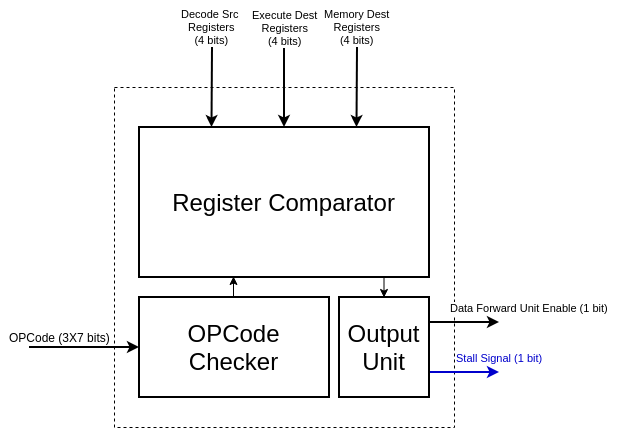
\includegraphics[width=0.8\textwidth]{hdu}
    \caption{Hazard Detection Unit Diagram}
    \label{fig:hdu}
\end{figure}

HDU consists of 3 parts:
\begin{itemize}
    \item \textbf{OPCode Checker:} checks the opcode of the current instruction to check whether it will cause data hazard or not, then activates the Register Comparator accordingly. Also, it checks for \emph{load-use case}, in order to activate the stall signal.
    \item \textbf{Register Comparator:} compares the decode source registers with the destination registers of the execute and memory stages.
    \item \textbf{Output Unit:} outputs stall signal in case of load and pop instructions and data forward unit enable in case of other data hazards.
\end{itemize}

\subsection{Handling}

\subsubsection{Stall}
Occurs only at Fetch and Decode stage, due to load(pop) use case.
\begin{itemize}
    \item Fetch same instruction (don't increment the program counter).
    \item Latch IF/ID buffer with the same values.
    \item Freeze Decode stage.
    \item Clear ID/EX buffer.
\end{itemize}

\subsubsection{Data Forwarding}
\begin{itemize}
    \item EX/MEM buffer $->$ Execute / Decode.
    \item ID/EX buffer $->$ Decode.
\end{itemize}

\section{Control Hazards}

\subsection{Detection}
The branch address calculation occurs in the Decode stage. So, the hazard might affect only the Fetch stage, which will be flushed in case of wrong address prediction.

\subsection{Handling}
\begin{itemize}
    \item At Fetch stage, always check the branch predictor and calculate the next address accordingly.
    \item At Decode stage, we have a \emph{Branch Address Unit} that checks whether the OPCode is of a branch operation. If so, it passes the address to the program counter and compares the correct address with the address of the counter to decide whether to flush the Fetch stage or not. 
\end{itemize}

\subsubsection{Flush}
Occurs only at Fetch Stage, due to wrong branch prediction at Decode stage.
\begin{itemize}
    \item Load new address in the program counter.
    \item Remove fetched instructions from IF/ID buffer.
\end{itemize}

\subsubsection{Dynamic Branch Prediction}
We use 2-bit branch predictor, which is a hash table of \emph{Finite State Machines} (FSMs) to predict whether the branch will be taken (1) or not (0) at each individual branch address.

\end{document}
